\section{Visualization}
\subsection{Research}

\begin{frame}{Visualization Research I}
% Academia hasn't innovated new methods in ages. Does try to speed things up.
% Noted in 2004, seems to still be true now.
% MET Office does 
% Our specific kind of visualization (in-situ visualization) emerged in the 2010s, but again this only focuses on speedup methods, hooking things together.
\begin{wideitemize}
    \item This program is an example of `tightly-coupled in-situ visualization' \parencite{kress2017situ}.
    \item Academia hasn't recently innovated in fluid visualization, only in methods for running faster such as \parencite{efficientStreamConstruction}.
    \item This was noted in \parencite{vizRole2004}, which states `feature detection' would be a key element going forward rather than new visualization methods.
\end{wideitemize}
\end{frame}

\begin{frame}{Visualization Research II}
\mytwocolumn{0.5}{
\begin{wideitemize}
    \item Industry seems to match this assessment.
    \item Tools such as Autodesk CFD, Tecplot, ParaView all visualize data with the same general methods...
    \item but they allow the data to be \emph{filtered} to extract relevant values.
    \item Methods can be combined to show a range of information.
\end{wideitemize}
}{
    \begin{figure}
        \centering
        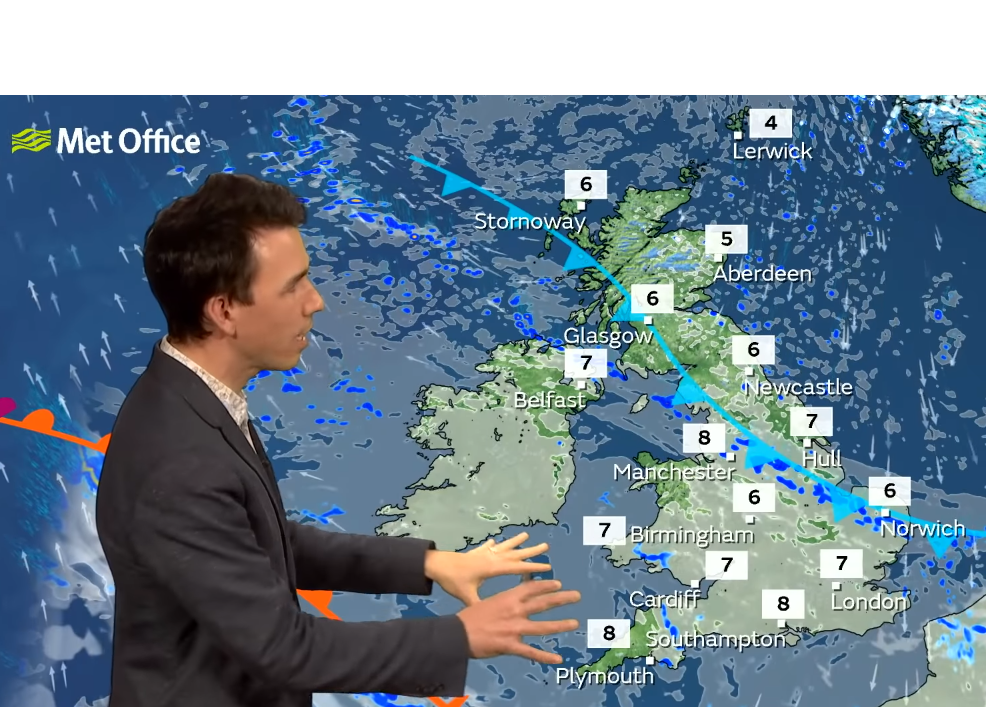
\includegraphics[width=0.7\textwidth]{Presentation/images/weather.PNG}
        \caption{Weather Forecast showing wind speed, weather fronts, and cloud cover.\footnotemark{}}
    \end{figure}
}
\footnotetext{\url{https://youtu.be/y_1--MkiNjQ}, Met Office 10 Day Trend for March 3rd.}
% Look to industry for potential innovation.
% Selected Autodesk CFD for a fluid-focused visualization.
% Found X methods of interest
% list them
% All have been present from 195X, confirming belief.
\end{frame}

\newcommand{\vizresearch}[3]{
\begin{frame}{Visualization Research}
    % \framesubtitle{What can Autodesk CFD do?}
    % \begin{columns}[t,onlytextwidth]
    %     \begin{column}{0.5\textwidth}
    %         {\Large #1}
    %         \vspace{2em}
    %         #2
    %     \end{column}
    %     \begin{column}{0.3\textwidth}
    %         #3
    %     \end{column}
    % \end{columns}
    
    \framesubtitle{What can Autodesk CFD do?}
    \begin{minipage}{0.5\textwidth}
        {\Large #1}
        \vspace{2em}
        #2
    \end{minipage}\hfill%
    \begin{minipage}{0.48\textwidth}
        #3
    \end{minipage}
\end{frame}
}

\vizresearch{Result Planes - Scalar}{
    % \todocite{http://help.autodesk.com/view/SCDSE/2019/ENU/?guid=GUID-AA40D02F-8CBC-4F78-A3C8-CEF30E05522B}
    \begin{wideitemize}
        \item Place a plane in 3D space
        \item Select a scalar quantity (pressure, temperature etc.)
        \item The cross-section of the model shows the selected quantity, with a color scale
        % \todomark{matplotlib jet colormap}
    \end{wideitemize}
}{
\begin{figure}
    \centering
    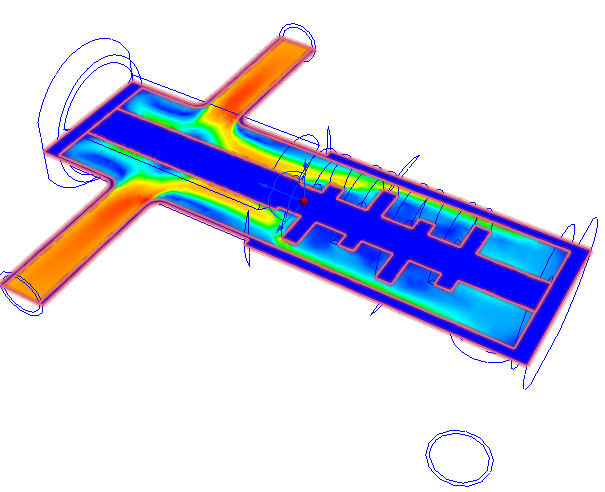
\includegraphics[width=0.9\textwidth]{Presentation/images/autodesk_cfd_results_planes_scalar.png}
\end{figure}
}

\vizresearch{Result Planes - Vector}{
    % \todocite{http://help.autodesk.com/view/SCDSE/2019/ENU/?guid=GUID-AA40D02F-8CBC-4F78-A3C8-CEF30E05522B}
    \begin{wideitemize}
        \item Place a plane in 3D space
        \item Select a \emph{vector} quantity (velocity etc.)
        \item The cross-section of the model shows a vector field of the selected velocity.
    \end{wideitemize}
}{
\begin{figure}
    \centering
    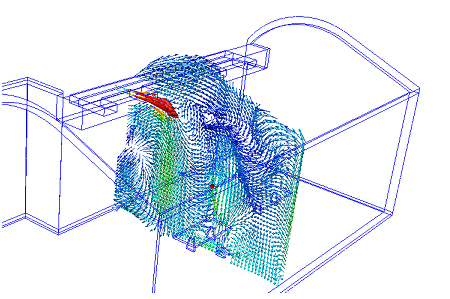
\includegraphics[width=0.9\textwidth]{Presentation/images/autodesk_cfd_results_planes_vector.png}
\end{figure}
}

\vizresearch{Isosurfaces}{
% \todocite{http://help.autodesk.com/view/SCDSE/2019/ENU/?guid=GUID-9D0D1D9C-C087-42A5-87F6-24F6A8530244}
    \begin{wideitemize}
        \item Select a scalar quantity $X$.
        \item Select a value $X = x$.
        \item This surface is displayed with a color based on another quantity $Y$.
        \item A vector quantity can also be added to the surface.
    \end{wideitemize}
}{
\begin{figure}
    \centering
    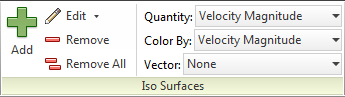
\includegraphics[width=0.6\textwidth]{Presentation/images/isosurface_control.png}
\end{figure}
\begin{figure}
    \centering
    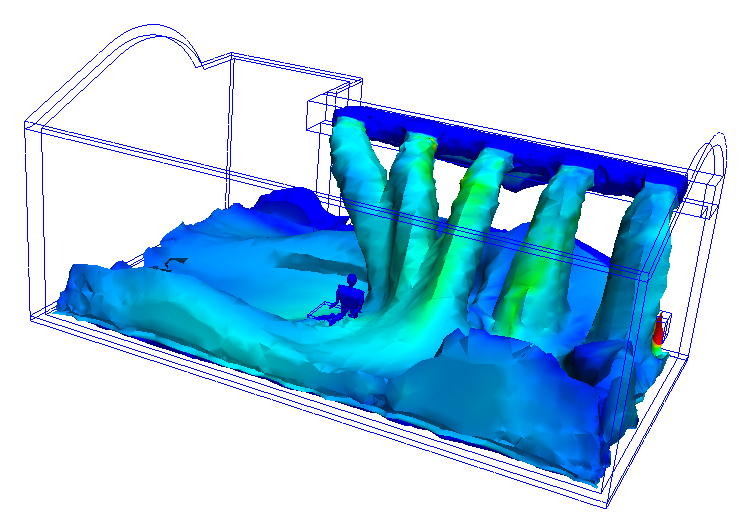
\includegraphics[width=0.9\textwidth]{Presentation/images/isosurface.png}
\end{figure}
}

\vizresearch{Isovolumes}{
% \todocite{http://help.autodesk.com/view/SCDSE/2019/ENU/?guid=GUID-9D0D1D9C-C087-42A5-87F6-24F6A8530244}
    \begin{wideitemize}
        \item Select a scalar quantity $X$.
        \item Select a \emph{range} $x_{min} \leq X \leq x_{max}$.
        \item This \emph{volume} is displayed with a color based on another quantity $Y$.
        \item A vector quantity can also be added to the \emph{volume}.
    \end{wideitemize}
}{
\begin{figure}
    \centering
    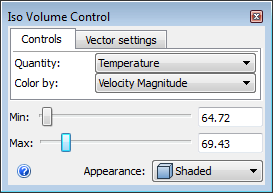
\includegraphics[width=0.5\textwidth]{Presentation/images/isovolume_ui.png}
\end{figure}
\begin{figure}
    \centering
    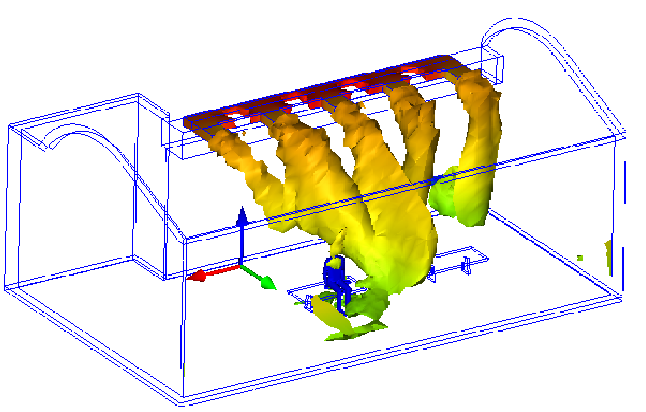
\includegraphics[width=0.9\textwidth]{Presentation/images/isovolume_noui.png}
\end{figure}
}

\vizresearch{Particles}{
% \todocite{http://help.autodesk.com/view/SCDSE/2019/ENU/?guid=GUID-9EBC3C73-AB3B-4341-BBDF-58601024BD7C}
    \begin{wideitemize}
        \item Place particle spawn points (`seeds').
        \item Select a scalar quantity to display, or a solid color.
        \item Points along the particle paths show the specified quantity.
        \item Can choose many kinds of path:
        \begin{itemize}
            \item Cylinders
            \item Ribbons
            \item Comets
            \item etc.
        \end{itemize}
    \end{wideitemize}
}{
\begin{figure}
    \centering
    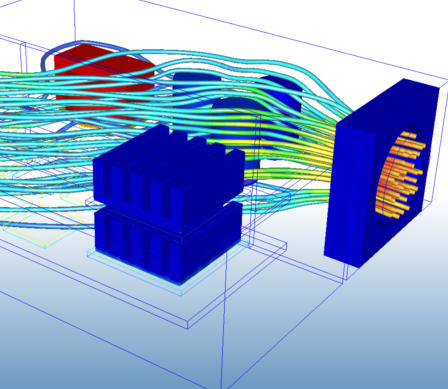
\includegraphics[width=0.9\textwidth]{Presentation/images/particle_traces.jpg}
\end{figure}
}

% \begin{frame}{Visualization Research II - Weather Reports}
% % Met office layers many effects on top of each other.
% \mytwocolumn{0.5}{
% \begin{wideitemize}
%     \item The MET office is an example of an intuitive fluid visualization.
%     \item 
% \end{wideitemize}
% }
% \end{frame}

\subsection{Design}

\begin{frame}{Selected Features}
% Select 3 layers, which can be overlayed on each other, like the weather report.

% Take iso-shapes as the 2D equivalent of isovolumes
% For both scalar and vector processing
% Add particles
%  failed to add particle trails
        Separate the visualization into layers:
        \vspace{1em}

        \begin{wideitemize}
            \item Background
            \item Scalar Quantity
            \begin{itemize}
                \item Display a quantity $X$ using a colormap when $x_{min} \leq X \leq x_{max}$
                \item Allow the user to select a range, or calculate a range containing all values
                \item Equivalent to Results Plane (Scalar) + 2D Isovolume
            \end{itemize}
            \item Vector Quantity 
            \begin{itemize}
                \item Display a vector field of $X$ when $x_{min} \leq X \leq x_{max}$
                \item Allow the user to select a range, or calculate a range containing all values
                \item Equivalent to Results Plane (Vector) + 2D Isovolume
            \end{itemize}
            \item Particles
                \begin{itemize}
                    \item Editable `seeds'
                    \item Planned for particle trace options, didn't have time.
                \end{itemize}
        \end{wideitemize}
    % }{
    % daui
    % }
\end{frame}

\begin{frame}{Anatomy of a Frame}
% "Mention zero copy"
% Need to mention "need compute + graphics"
% Include CPU recording

    \makebox[\textwidth][c]{
    \begin{tikzpicture}[
    scale=0.9, every node/.style={scale=0.9},
fixedrect/.style={rectangle,draw,minimum height=4em,anchor=west,text width=2cm,align=center},
]
        \node[label=west:{GPU},align=right](gpu) at (0,0){};
        \node[label=west:{CPU 0},align=right](c0) at (0,-4em){};
        \node[label=west:{CPU 1},align=right](c1) at (0,-8em){};

        \node[fixedrect, text width=1.5cm, path fading = west](gpu_viz_g_old) at (gpu){Viz \\N-1};%\\[Vulkan]};
        \node[fixedrect, text width=6cm](gpu_sim) at (gpu_viz_g_old.east){Simulation\\N};%\\[CUDA]};
        \node[fixedrect, text width=2cm](gpu_viz_c) at (gpu_sim.east){Viz Compute\\N};%\\[Vulkan]};
        \node[fixedrect, text width=2cm](gpu_viz_g) at (gpu_viz_c.east){Viz Graphics\\N};%\\[Vulkan]};
        \node[fixedrect, text width=2cm, path fading = east](gpu_sim_next) at (gpu_viz_g.east){Sim\\N+1};%\\[Vulkan]};

        \node[fixedrect, text width=4.5cm](c0_sim) at (c0 -| gpu_sim.west){Launch Sim Kernels};%\\[Vulkan]};
        \node[fixedrect, text width=3cm](c1_record) at (1,0 |- c1){Record Visualization};%\\[Vulkan]};

        % \draw[-latex] (c0_sim.north -| 1,0) -- (gpu_sim.west);
        \draw[-latex] (c1_record.east) -| (gpu_viz_c.south west);
        \draw[-latex] (c0) -- (c1_record.west);
        % \draw[-latex] (c1_record.east) -- (gpu_viz.south);
        % \draw[-latex] (c1_record.east) -| (gpu_viz.south);
        % \draw[-latex] (c1_record.east) -| (gpu_viz.south);
    \end{tikzpicture}
    }

    \vfill\null
    \begin{wideitemize}
        % \item CPU 0 (main thread) starts a worker thread to record what the GPU will do for the visualization.
        \item CPU 0 launches the simulation, which requires some CPU/GPU sync at the start.
        \item CPU 1 enqueues the visualization work to start right after the simulation.
        \item Sim and Visualization share memory, architecture is zero-copy.
        \item Maintains near-100\% GPU Utilization.
    \end{wideitemize}
    % Key point is that the "Record Visualization" may overlap with a previous viz frame, so it can't look at any GPU memory.
\end{frame}

\begin{frame}{GPU Synchronization}
% Semaphores
    \makebox[\textwidth][c]{
    \begin{tikzpicture}[
            scale=0.9, every node/.style={scale=0.9},
        fixedrect/.style={rectangle,draw,minimum height=4em,anchor=west,text width=2cm,align=center},
        ]
        \node[label=west:{GPU - CUDA},align=right](cuda) at (0,0){};
        \node[label=west:{GPU - Vulkan},align=right](vulkan) at (0,-4em){};

        \node[fixedrect, text width=1.5cm, path fading = west](vc_old) at (vulkan){Viz Comp\\N-1};
        \node[fixedrect, text width=2cm](vg_old) at (vc_old.east){Viz Graphics\\N-1};
        \node[fixedrect, text width=6cm](sim) at (vc_old.east |- cuda){Simulation\\N};%\\[CUDA]};
        \node[fixedrect, text width=2cm](vc) at (sim.east |- vulkan){Viz Compute\\N};%\\[Vulkan]};
        \node[fixedrect, text width=2cm](vg) at (vc.east){Viz Graphics\\N};
        \node[fixedrect, text width=4cm, anchor=west,path fading = east](sim_new) at (vg.west |- cuda){Sim\\N+1};
        
        \draw[ultra thick,black,-Triangle] (vc.south west) -- (sim.north east) |- ++(0.25,0.5) ;
            % node[east,text width=2cm,anchor=west]{Vulkan/CUDA Shared Semaphore};
        \draw[ultra thick,black,-Triangle] (vc_old.south east) -- (sim.north west) |- ++(0.25,0.5) ;
            % node[east,text width=2cm,anchor=west]{Vulkan/CUDA Shared Semaphore};
        \draw[ultra thick,black,-Triangle] (vg.south west) -- (sim_new.north west) |- ++(0.25,0.5) ;
            % node[east]{};
            
        % \draw[ultra thick,black,-Triangle] (vg.south west) -- (vg.north west) |- ++(0.25,0.5) ;
            % node[text width=2cm,anchor=north,below=5pt]{Vulkan-Only};

            
        % \node[text width = 3cm,align=center,anchor=north,below=10pt](sem_label) at (sim.south |- vc.south){Vulkan/CUDA Shared};
        % \draw[dashed](sem_label.north east) -- (vc.south west);
        % \draw[dashed](sem_label.north west) -- (vg_old.south east);
        
        % \node[text width = 3cm,align=center,anchor=north,below=10pt](vk_label) at (vg.south west){Vulkan-Only};
        % \draw[dashed](vk_label.north) -- (vc.south east);

        \end{tikzpicture}
    }

    \vfill\null
    
    \begin{wideitemize}
        \item Synchronization between overall workloads is performed via \emph{semaphores}\footnote{\url{https://www.khronos.org/registry/vulkan/specs/1.2-extensions/man/html/VkSemaphore.html}}.
        \item One workload waits on a semaphore until another workload signals it.
        \item Compute workloads cannot overlap on my graphics card\footnote{Running parallel compute workloads was introduced in \parencite{nvidiaAmpereWhitepaper}}
        \item Simulation and Viz Graphics \emph{could} overlap, but don't in practice.
        % \item More semaphores used in the program for `present' logic.
    \end{wideitemize}
\end{frame}

\begin{frame}{GPU Synchronization - Less Misleading}
% Semaphores
    \makebox[\textwidth][c]{
    \begin{tikzpicture}[
            scale=0.9, every node/.style={scale=0.9},
        fixedrect/.style={rectangle,draw,minimum height=4em,anchor=west,text width=2cm,align=center},
        ]
        \node[label=west:{GPU - CUDA},align=right](cuda) at (0,0){};
        \node[label=west:{GPU - Vulkan},align=right](vulkan) at (0,-4em){};

        \node[fixedrect, text width=1.5cm, path fading = west](vc_old) at (vulkan){Viz Comp\\N-1};
        \node[fixedrect, text width=2cm](vg_old) at (vc_old.east){Viz Graphics\\N-1};
        \node[fixedrect, text width=6cm](sim) at (vc_old.east |- cuda){Simulation\\N};%\\[CUDA]};
        \node[fixedrect, text width=2cm](vc) at (sim.east |- vulkan){Viz Compute\\N};%\\[Vulkan]};
        \node[fixedrect, text width=2cm](vg) at (vc.east){Viz Graphics\\N};
        \node[fixedrect, text width=4cm, anchor=west,path fading = east](sim_new) at (vg.west |- cuda){Sim\\N+1};
        
        \draw[ultra thick,black,-Triangle] (vc.south west) -- (sim.north east) |- ++(0.25,0.5) ;
            % node[east,text width=2cm,anchor=west]{Vulkan/CUDA Shared Semaphore};
        \draw[ultra thick,black,-Triangle] (vc_old.south east) -- (vc_old.east) -- (sim_new.west) -- (sim_new.north west) |- ++(0.25,0.5) ;
            % node[east,text width=2cm,anchor=west]{Vulkan/CUDA Shared Semaphore};
        \draw[ultra thick,black,-Triangle] (vg.south west) -- (vg.north west) |- ++(0.25,0.2) ;
            % node[east]{};
            
        % \draw[ultra thick,black,-Triangle] (vg.south west) -- (vg.north west) |- ++(0.25,0.5) ;
            % node[text width=2cm,anchor=north,below=5pt]{Vulkan-Only};

            
        % \node[text width = 3cm,align=center,anchor=north,below=10pt](sem_label) at (sim.south |- vc.south){Vulkan/CUDA Shared};
        % \draw[dashed](sem_label.north east) -- (vc.south west);
        % \draw[dashed](sem_label.north west) -- (vg_old.south east);
        
        % \node[text width = 3cm,align=center,anchor=north,below=10pt](vk_label) at (vg.south west){Vulkan-Only};
        % \draw[dashed](vk_label.north) -- (vc.south east);

        \end{tikzpicture}
    }

    \vfill\null
    
    \begin{wideitemize}
        \item Synchronization between overall workloads is performed via \emph{semaphores}\footnote{\url{https://www.khronos.org/registry/vulkan/specs/1.2-extensions/man/html/VkSemaphore.html}}.
        \item One workload waits on a semaphore until another workload signals it.
        \item Compute workloads cannot overlap on my graphics card\footnote{Running parallel compute workloads was introduced in \parencite{nvidiaAmpereWhitepaper}}
        \item Simulation and Viz Graphics \emph{could} overlap, but don't in practice.
        % \item More semaphores used in the program for `present' logic.
    \end{wideitemize}
\end{frame}

\subsection{Implementation}

\begin{frame}[fragile]{Extracting Simulation Data}
% `ask me about this later' slide

    \begin{minipage}{0.48\textwidth}
       \begin{wideitemize}
            \item First part of Viz Compute.
            \item Transfer + interpolate data from 1D arrays to a 2D texture.
            \item More complex than a simple copy. % NOTE - have to change coordinate spaces too.
            \item Allows arbitrary sampling, using built-in texture filtering for free interpolation.
        \end{wideitemize}
    \end{minipage}\hfill%
    \begin{minipage}{0.5\textwidth}
    \lstset{language=glsl}
        \begin{lstlisting}
float u[], v[], p[], isfluid[];

int idx = i * pConsts.height + j;
vec2 velocity = vec2(u[idx], v[idx]);\end{lstlisting}

        \makebox[\textwidth][c]{
            \begin{tikzpicture}
                \draw[-latex] (0,0) -- (0, -0.5);
            \end{tikzpicture}
        }
        
        \begin{lstlisting}
uniform sampler2D simDataSampler;
 // = (u, v, p, isfluid);
 
 // 50% across, 20% up the image
vec2 sampleAt = (0.5, 0.2);
vec2 velocity = 
    texture(simDataSampler, sampleAt).xy;\end{lstlisting}

    \end{minipage}
    

    \vfill\null
    \begin{center}
        \hyperlink{frame:simdatatex}{Ask me about Simulation Data Textures at the end!}
    \end{center}
\end{frame}

\newcommand{\tikzstaggeredgrid}[1]{
    \draw[#1] (0, 1) -- (6, 1);
    \draw[#1] (0, 3) -- (6, 3);
    
    \draw[#1] (1,4) -- (1,0);
    \draw[#1] (3,4) -- (3,0);
    \draw[#1] (5,4) -- (5,0);
    
    % \node at (0, 0.5) {j-1}; 
    % \node at (0, 2) {j}; 
    % \node at (0, 3.5) {j+1};
    
    % \node at (0.5, 0) {i-1}; 
    % \node at (2, 0) {i}; 
    % \node at (4, 0) {i+1};
    % \node at (5.5, 0) {i+2};
    
    \node[label=above:{$p_{i,j}$}, draw, circle, fill, minimum size=0.12cm, inner sep=0pt] at (2, 2) {};
    \node[label=above:{$p_{i+1,j}$}, draw, circle, fill, minimum size=0.12cm, inner sep=0pt] at (4, 2) {};
    
    \node[label=below left:{$u_{i-1,j}$}, draw, diamond, fill, minimum size=0.14cm, inner sep=0pt] at (1, 2) {};
    \node[label=below left:{$u_{i,j}$}, draw, diamond, fill, minimum size=0.14cm, inner sep=0pt] at (3, 2) {};
    \node[label=below right:{$u_{i+1,j}$}, draw, diamond, fill, minimum size=0.14cm, inner sep=0pt] at (5, 2) {};
    
    \node[label=above:{$v_{i,j}$}, draw, rectangle, fill, minimum size=0.1cm, inner sep=0pt] at (2, 3) {};
    \node[label=above:{$v_{i+1,j}$}, draw, rectangle, fill, minimum size=0.1cm, inner sep=0pt] at (4, 3) {};
    \node[label=below:{$v_{i,j-1}$}, draw, rectangle, fill, minimum size=0.1cm, inner sep=0pt] at (2, 1) {};
    \node[label=below:{$v_{i+1,j-1}$}, draw, rectangle, fill, minimum size=0.1cm, inner sep=0pt] at (4, 1) {};
}
\begin{subframe}{Simulation Data Texture}
\label{frame:simdatatex}
    \begin{wideitemize}
        \item Simulation stores data points from a staggered grid.
        \item Visualization wants to get data at arbitrary locations, which texture hardware is really good at.
        \item Convert the original data to a texture 2x the resolution, and interpolate when values aren't present.
    \end{wideitemize}
% }{
    \begin{center}
        \begin{tikzpicture}[scale=0.8,every node/.style={scale=0.8},]
            \tikzstaggeredgrid{}
            
            \draw[->](6.5, 2) -- (7.5, 2);
            
            \begin{scope}[shift={(8,0)},every label/.append style={text opacity=0}]
                \tikzstaggeredgrid{dashed,opacity=0.2}
                
                \draw[red] (0, 0.5) -- (6, 0.5);
                \draw[red] (0, 1.5) -- (6, 1.5);
                \draw[red] (0, 2.5) -- (6, 2.5);
                \draw[red] (0, 3.5) -- (6, 3.5);

                \draw[red] (1.5,4) -- (1.5,0);
                \draw[red] (2.5,4) -- (2.5,0);
                \draw[red] (3.5,4) -- (3.5,0);
                \draw[red] (0.5,4) -- (0.5,0);
                \draw[red] (4.5,4) -- (4.5,0);
                \draw[red] (5.5,4) -- (5.5,0);
            \end{scope}
        \end{tikzpicture}
    \end{center}
\end{subframe}

\newcommand{\perlayervizwork}{
    \node[label=west:{Scalar Quantity},align=right](sq) at (0,0){};
    \node[label=west:{Vector Quantity},align=right](vq) at (0,-1.5){};
    \node[label=west:{Particles},align=right](p) at (0,-3){};
    
    % \node[fixedrect](sq_prelim) at (0, 1){Convert arrays to image};
    \node[fixedrect](sq_c1) at (sq){Extract Quantity};
    \node[fixedrect](sq_c2) at (sq_c1.east){Find min/max\\(Optional)};
    
    \node[fixedrect](vq_c1) at (vq){Extract Quantity};
    \node[fixedrect](vq_c2) at (vq_c1.east){Find min/max\\(Optional)};
    \node[fixedrect](vq_c3) at (vq_c2.east){Create Vector Instances};
    
    \node[fixedrect](p_c1) at (p){Decide Particles to emit};
    \node[fixedrect](p_c2) at (p_c1.east){Emit new Particles};
    \node[fixedrect](p_c3) at (p_c2.east){Simulate Particles};
    
    \node[fixedrect](sq_r) at (10.5, 0){Draw\\Background w/ Quantity};
    \node[fixedrect](vq_r) at (sq_r.west |- vq){Draw\\Vector Instances};
    \node[fixedrect](p_r) at (sq_r.west |- p){Draw\\Particles};
    
    \draw [decorate,decoration={brace,raise=5pt,amplitude=7pt,mirror},yshift=-20pt](sq_c1.west |- p_r.south) -- (p_c3.east |- p_r.south) node [black,midway,anchor=north,below=15pt]{Compute};
    
    \draw [decorate,decoration={brace,raise=5pt,amplitude=7pt,mirror},yshift=-20pt](sq_r.west |- p_r.south) -- (p_r.east |- p_r.south) node [black,midway,anchor=north,below=15pt]{Graphics};
}

\begin{frame}{Per-Layer Viz Work}
    \makebox[\textwidth][c]{
        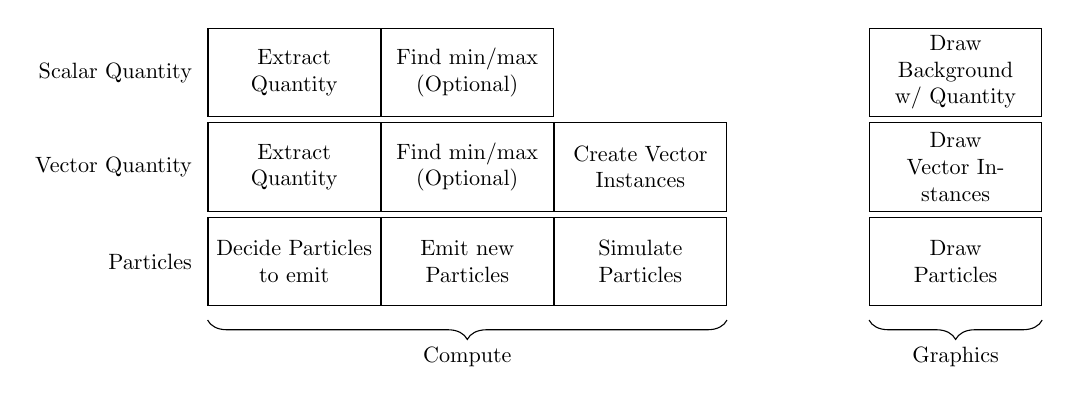
\begin{tikzpicture}[
            scale=0.8, every node/.style={scale=0.8},
            fixedrect/.style={rectangle,draw,minimum height=4em,anchor=west,text width=2.5cm,align=center},
        ]   
            \perlayervizwork{}
        \end{tikzpicture}
    }
    
    \vfill\null
    
    \begin{wideitemize}
        % \item Each of the squares here represents a Pipeline.%\todocite{Vulkan spec on pipelines??}
        \item Compute Pipelines use one Compute Shader, roughly equivalent to CUDA Kernels.
        \item Graphics Pipelines use a Vertex Shader and a Fragment Shader to draw to a render target.
        \item There is also a `final composite' stage which renders the GUI with the viz output.
    \end{wideitemize}
\end{frame}

\begin{frame}{Viz Compute Order}
    \makebox[\textwidth][c]{
        \begin{tikzpicture}[
            scale=0.9, every node/.style={scale=0.9},
            fixedrect/.style={rectangle,draw,minimum height=4em,anchor=west,text width=2cm,align=center},
            barrier/.style={rectangle,draw,minimum height=4em,anchor=west,minimum width=0.2cm,pattern=south west lines}
        ]
        
            \node[fixedrect](prelim) at (0,-5em){Extract Sim Data Texture};
            \node[barrier](prelim_b) at (prelim.east){};
            \node[fixedrect](sq1) at (prelim_b.east){Extract Scalar Quantity};
            \node[barrier](sq1_b) at (sq1.east){};
            \node[fixedrect](sq2) at (sq1_b.east){Find Scalar min/max};
            \node[barrier](sq2_b) at (sq2.east){};
            \node[fixedrect](vq1) at (sq2_b.east){Extract Vector Quantity};
            \node[barrier](vq1_b) at (vq1.east){};
            \node[fixedrect](vq2) at (vq1_b.east){Find Vector min/max};
            \node[barrier](vq2_b) at (vq2.east){};
            \node[fixedrect](vq3) at (vq2_b.east){Create Vector Instances};
            % \node[fixedrect](p1) at (vq3.east){etc.};

        
            \draw [decorate,decoration={brace,raise=5pt,amplitude=7pt,mirror},yshift=-20pt](sq1.south west) -- (sq2.south east) node [black,midway,anchor=north,below=15pt]{Scalar Quantity};
            \draw [decorate,decoration={brace,raise=5pt,amplitude=7pt,mirror},yshift=-20pt](vq1.south west) -- (vq3.south east) node [black,midway,anchor=north,below=15pt]{Vector Quantity};
            % \draw [decorate,decoration={brace,raise=5pt,amplitude=7pt,mirror},yshift=-20pt](p1.south west) -- (p1.south east) node [black,midway,anchor=north,below=15pt]{};
            % \draw (vc_overall.south west) -- (vc1.north west);
            
            \node[fixedrect,
            rectangle split,
            rectangle split parts=2,
            rectangle split horizontal,
            rectangle split draw splits=false,
            text width=7cm](vc_overall) at (0,0){Viz Compute\nodepart{two}};%\\[Vulkan]};
            \begin{scope}[overlay]
                \node[fixedrect,fill=white,draw=white,path fading=west,minimum width=2cm,anchor=east,minimum height=50em](fade) at (13cm,0){};
                \node[fixedrect,fill=white,draw=white,minimum width=2cm,anchor=west,minimum height=50em] at (fade.east){};
            \end{scope}
        \end{tikzpicture}
    }
    
    \vfill\null
    
    \begin{wideitemize}
        % \item Each of the squares here represents a Pipeline.%\todocite{Vulkan spec on pipelines??}
        \item Computer work for layers is done serially, not in parallel (which could be improved in the future).
        \item Vulkan uses Execution and Memory Barriers to ensure ordering. (Ask me about this at the end!)
        \item Vectors and Particles are drawn with Indirect Instanced rendering.
    \end{wideitemize}
\end{frame}

\begin{frame}{Indirect Instanced Rendering}
% ask me about this afterwrads!

        % \makebox[\textwidth][c]{
    % \begin{tikzpicture}[
    %     scale=0.8, every node/.style={scale=0.8},
    %     indirectrect/.style={rectangle,draw,minimum height=4em,anchor=north west,text width=2.5cm,align=center},
    % ]   
    %     % \node[indirectrect, text width=6cm, minimum height=2em](inst_fill) at (0,0) {CPU or GPU generates data};
    %     \node[indirectrect, minimum height = 8em,text width=2cm](inst_data) at (4,-1.5) {8\\Positions};
    %     \node[indirectrect, anchor=south west](inst_draw) at (0,0 |- inst_data.south) {Render 8 things\\at positions};
        
    %     % \draw[-latex] (inst_fill) -- (inst_data.north);
    %     \draw[-latex] (inst_data) -- (inst_draw.east);
        
    %     \node[text width=5cm] at (4, -4.7) {Instanced Rendering};

    %     \begin{scope}[shift={(8,0)},every label/.append style={text opacity=0}]
    %         \node[indirectrect](indirect_fill) at (0,0) {Compute Shader\\generates data};
    %         \node[indirectrect, minimum height = 1em,text width=2cm](indirect_len) at (4,-1.5) {N = 7};
    %         \node[indirectrect, minimum height = 7em,text width=2cm](indirect_data) at (indirect_len.south west){7+\\Positions};
    %         \node[indirectrect, anchor=south west](indirect_draw) at (0,0 |- indirect_data.south) {Render N things\\at positions};
            
    %         \draw[-latex] (indirect_fill.east) -- (indirect_len.north);
    %         \draw[-latex] (indirect_len.west) -- (indirect_draw.north);
    %         \draw[-latex] (indirect_data) -- (indirect_draw.east);
            
    %         \node[text width=5cm] at (4, -4.7) {Indirect Instanced Rendering};
    %     \end{scope}
    % \end{tikzpicture}
    % }
    
        \makebox[\textwidth][c]{
    \begin{tikzpicture}[
    scale=0.9, every node/.style={scale=0.9},
fixedrect/.style={rectangle,draw,minimum height=4em,anchor=west,text width=2cm,align=center},
]
        \node[label=west:{GPU},align=right](gpu) at (0,0){};
        \node[label=west:{},align=right](memory) at (0,-6em){};

        \node[fixedrect](instanced_draw) at (gpu){Draw 8 particles};
        \node[fixedrect](instanced_data) at (instanced_draw.west |- memory){Positions of 8 particles};
        
        \node[fixedrect](indirect_compute) at ($(gpu) + (5, 0)$){Simulate ??? particles};
        \node[fixedrect](indirect_draw) at ($(indirect_compute.west) + (5cm,0)$){Draw N particles};
        \node[fixedrect, text width = 7cm](indirect_data) at (indirect_compute.west |- memory){N = 24\\Positions of 24+ particles};
        
        \draw[-latex] (instanced_data.north) -- (instanced_draw.south) node[right,midway]{read};

        \draw[-latex] (indirect_compute.south) -- (indirect_compute.south |- indirect_data.north) node[right,midway]{write};
        \draw[-latex] (indirect_draw.south |- indirect_data.north) -- (indirect_draw.south)  node[right,midway]{read};

        \draw ($(instanced_draw.north west) + (-0.5,0)$) -- ($(indirect_draw.north east) + (0.5,0)$);
        \draw ($(instanced_draw.south west) + (-0.5,0)$) -- ($(indirect_draw.south east) + (0.5,0)$);
        
        \draw [decorate,decoration={brace,raise=5pt,amplitude=7pt,mirror},yshift=-20pt](instanced_data.south west) -- (instanced_data.south east) node [black,midway,anchor=north,below=15pt]{Instanced Rendering};
        
        \draw [decorate,decoration={brace,raise=5pt,amplitude=7pt,mirror},yshift=-20pt](indirect_data.south west) -- (indirect_data.south east) node [black,midway,anchor=north,below=15pt]{Indirect Instanced Rendering};

        % \node[fixedrect, text width=6cm](gpu_sim) at (gpu_viz_g_old.east){Simulation\\N};%\\[CUDA]};
        % \node[fixedrect, text width=2cm](gpu_viz_c) at (gpu_sim.east){Viz Compute\\N};%\\[Vulkan]};
        % \node[fixedrect, text width=2cm](gpu_viz_g) at (gpu_viz_c.east){Viz Graphics\\N};%\\[Vulkan]};
        % \node[fixedrect, text width=2cm, path fading = east](gpu_sim_next) at (gpu_viz_g.east){Sim\\N+1};%\\[Vulkan]};

        % \node[fixedrect, text width=4.5cm](c0_sim) at (c0 -| gpu_sim.west){Launch Sim Kernels};%\\[Vulkan]};
        % \node[fixedrect, text width=3cm](c1_record) at (1,0 |- c1){Record Visualization};%\\[Vulkan]};

        % % \draw[-latex] (c0_sim.north -| 1,0) -- (gpu_sim.west);
        % \draw[-latex] (c1_record.east) -| (gpu_viz_c.south west);
        % \draw[-latex] (c0) -- (c1_record.west);
        % % \draw[-latex] (c1_record.east) -- (gpu_viz.south);
        % % \draw[-latex] (c1_record.east) -| (gpu_viz.south);
        % % \draw[-latex] (c1_record.east) -| (gpu_viz.south);
    \end{tikzpicture}
    }

    \vfill\null
    \begin{wideitemize}
        \item We don't know how many Vectors/Particles exist at record time.
        \item Tell the GPU to look somewhere in memory to find how many copies to render.
    \end{wideitemize}
    \vfill\null
    \begin{center}
        Ask me about indirect/instanced/indexed rendering at the end!
    \end{center}
\end{frame}


\begin{frame}{Result!}
\makebox[\textwidth][c]{
    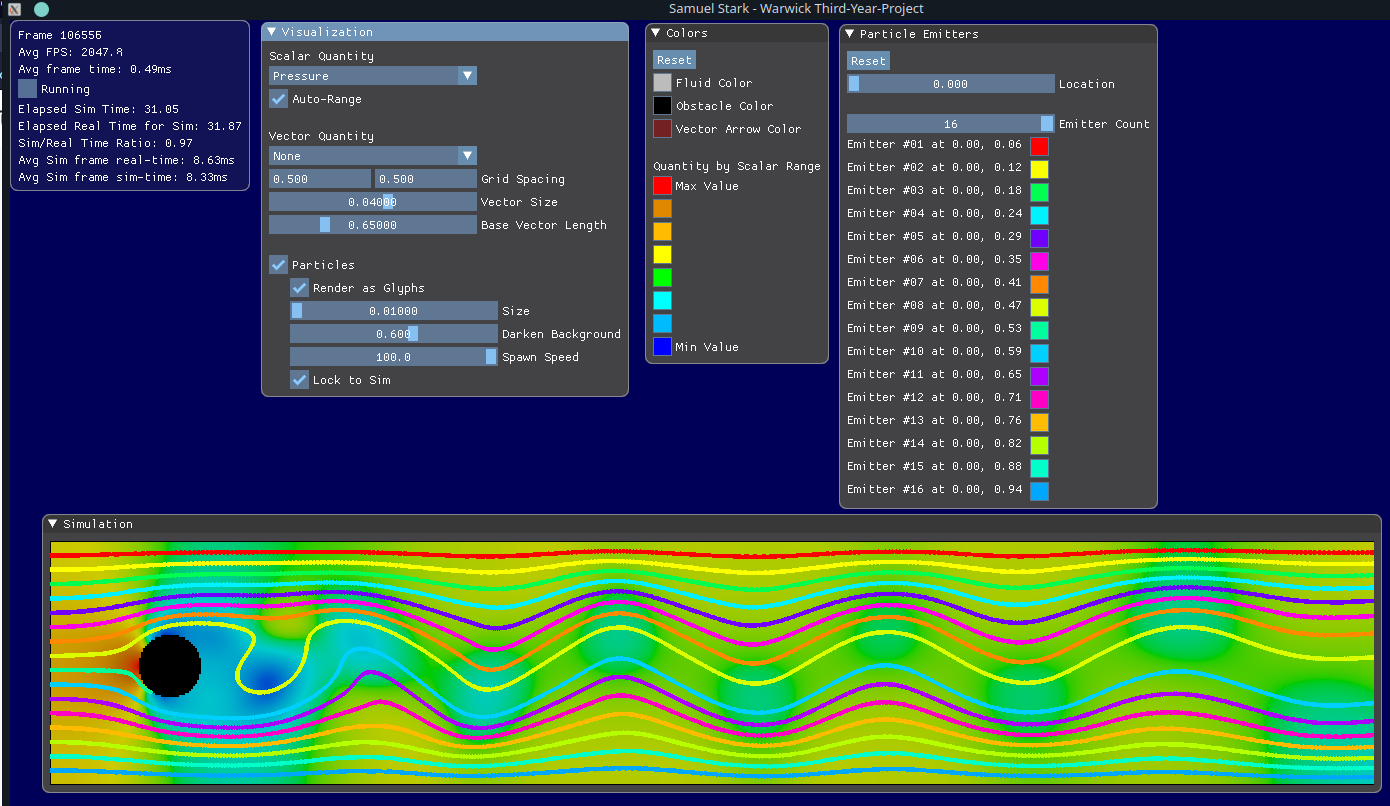
\includegraphics[width=0.8\textwidth]{Presentation/images/dan.png}
}
\end{frame}